%*******************************************************
%                       EINLEITUNG  
%*******************************************************
\chapter[Einleitung]{\label{sec:Einleitung}Einleitung}
% max 1 Seite
Mit den aktuellen Herausforderungen bei der Reduzierung von Treibhausgasen~\cite{MacDowell2017} steigt das Interesse an Energiespeicherkonzepten, die den Weg für energieeffiziente und nachhaltige Systeme ebnen~\cite{Owusu2016}. Im Kontext dieses Wandels besteht ein Teilaspekt im Übergang von ineffizienten fossilen Antriebssystemen zu effizienteren elektrischen Antrieben~\cite{Sugiyama2012}. Zur Versorgung dieser Systeme mit elektrischer Energie gibt es mehrere vielversprechende Konzepte, wie etwa Brennstoffzellen, Superkondensatoren und Batterien~\cite{Winter2004,Hemmati2016,Salkuti2023}. Besonders Letztere haben sich bei der Verwendung in mobilen Systemen, wie etwa elektrischen Fahrzeugen~\cite{Huo2015,Donateo2015,Jochem2015,Kim2014,Orsi2016,Silva2011,Holdway2010,Sternberg2015,Ramachandran2015}, Flugdrohnen~\cite{VincentWong2015,Boukoberine2019,Pham2022,Wang2022} und mobilen Robotern~\cite{Hecht2023,Mikolajczyk2023,Ghobadpour2023,Wang2020}, wegen ihrer hohen Energiedichte vielfach bewährt.

Allerdings ist bereits abzusehen, dass für zukünftige Anwendungen der Energiebedarf weiter ansteigt~\cite{Foiadelli2018}. Daher müssen Lösungen gefunden werden, wie die Menge an gespeicherter elektrischer Energie effizienter in ein System integriert werden kann~\cite{VanMierlo2007,Xu2022}.
%Ansätze, wie etwa Optimierung der Zellchemie werden aktuell zwar viel untersucht, stoßen aber langfristig an thermodynamische Grenzen~\cite{Zu2011,Njema2024}. Diese Grenzen sorgen dafür, dass das Optimierungspozenzial auf Zellebene mit den bisher bekannten Stoffen auf 5216,9~$\si{\watt\hour\per\kg}$ begrenzt ist, was eine zwölffache Steigerung gegenüber heutigen Batterien darstellt. 
Hierbei kann ausgenutzt werden, dass Batterien bisher nur wenig mechanisch belastbar sind und deshalb häufig mit einer zusätzlichen Schutzstruktur umgeben sind. Hinzu kommt, dass durch die klare Funktionsteilung keine synergetischen Effekte genutzt werden können, wie z.~B. bei Materialien, die sowohl als Energiespeicher als auch als Strukturkomponente dienen können. Der daraus resultierende Massenanteil von Materialien, die keinen Beitrag zur Energiespeicherung leisten, beträgt bei eingebauten Batteriepacks, wie der Audi Q4 e-tron Reihe, etwa 40~\% \cite{Radu2021,Audi2022}. Das daraus resultierende niedrige Verhältnis von Energiespeicher zu Masse des Gesamtsystems ist eine der größten Schwächen dieser Technologie \cite{Armand2020,Schaefer2018,Cano2018,Goodenough2009}. %, siehe Anhang~\ref{ch:AudiEnergie}. %Gesamtenergiedichte von 37~kWh/kg. Der Grenzwert für den Nutzen im Bereich des elektrischen Fliegens liegt nach \textsc{Scholz et al.} bei 51.8~Wh/kg \cite{Scholz2018}.

Ein vielversprechender Ansatz stellt daher die Entwicklung von Verbundstrukturen dar, die neben ihrer, auf Interkalation basierenden, elektrischen Speicherung auch mechanische Lasten in einem signifikanten Umfang aufnehmen können~\cite{Wong2007,Carlson2013}. Die bisherigen Forschungsarbeiten zu diesen, häufig auch als Strukturbatterien bezeichneten, Verbundstrukturen~\cite{Johannisson2018,Liu2009,Ekstedt2010,Wang2019,Zhao2020,Yin2020,Lutkenhaus2020,Fu2021,Jin2021,Kalnaus2021} nähern sich bereits dem Punkt, an dem relevante Einsparungen bei der Gesamtmasse und dem Gesamtvolumen realisiert werden können~\cite{Wetzel2004,Snyder2015,Carlstedt2020a,Asp2014,Johannisson2019}. Auch zeigen sich bereits weitere Vorteile, wie etwa die leichtere Integration in bestehende Designs, wodurch die Gewichtsverteilung erleichtert wird und ein Einbau näher am Verbraucher ermöglicht wird, was wiederum die Einsparung von Kabeln erlaubt~\cite{Thomas2004,Danzi2021,Moyer2020,Wang2020}. %Diese Vorteile erlauben neue innovative Designs im Bereich Elektrofahrzeuge, elektrische Alltagsgeräte wie etwa Laptops und Telefone, mobile Roboter, Flugdrohnen und Satelliten.

Das noch sehr junge Alter dieses Forschungsbereiches und der bisherige Fokus auf nur eine geringe Anhanzahl verschiedener Zellchemien lassen großes Optimierungspotenzial in bisher unerforschten Materialkombinationen vermuten~\cite{Asp2019}. Auf die Identifizierung neuer geeigneter Strukturbatterien für laminare Bauweisen mittels computergestützter Analysen fokussiert sich diese Dissertation.
Die hier dargestellte Forschung ist Teil der vom Deutschen Bundestag geförderten Forschungsinitiative „Luftfahrtforschung und -technologie“ LuFo-VI-2 in der Programmlinie „(A) Disruptive Technologien und innovative Systeme (ökoeffizientes Fliegen)“ im Fachbereich „(4) Strukturen und Bauweisen“ mit dem wichtigsten förderpolitischen Ziel „umweltfreundliche Luftfahrt“. Dies geschieht im Rahmen der „Entwicklung und Erprobung ultraleichter Verbundstrukturen mit integrierter elektrischer Speicherfunktion“ (ElViS).


%*************************************************************
%               Motivation und Zielstellung  
%*************************************************************
\section{\label{sec:Motivation_Zielstellung}Problemstellung und Zielsetzung}
% rund 1,5 Seiten inklusive Bild

%Um die Reichweite und Nutzungsdauer von mobilen elektrischen Geräten, wie Elektrofahrzeuge und mobile Roboter zu erhöhen ist sind elektrische Speicher mit besserem Verhältnis von Speichervermögen zu Gesamtmasse von entscheidenter Bedeutung. Aus dieser übergeordneten Zielstellung leiten sich drei mögliche Ansätze ab: erstens die Energiedichte der einzelnen Speicherzellen steigern, zweitens die Masse der mechansichen Entkoppelung durch die Verwendung von Werkstoffen mit hoher spezifischer Festigkeit und Steifigkeit reduzieren und drittens die Erhöhung der Gesamtenergiedichte durch die Verwendung von mechanisch belastbaren Batterien, welches einen Kompromiss zu den ersten beiden Ansätzten darstellt.

%Der letzte Ansatz hat außerdem den Vorteil, dass solche strukturtragenden Batterien (kurz Strukturbatterien) flexibler verbaut werden können und somit bei Verkabelung eingespart werden kann und Gewichtsverteilungsprobleme, wie sie etwa bei Flugmaschinen und Satelliten auftreten einfacher gelöst werden können
Um zukünfitg in Satelitentechnik, Roboteren und der Elektomonilitätsbranche eingesetzt zu werden müssen Strukturbatterien gegenüber einem konventionellen Batterie-Kohlefaserverbund einen Massenvorteil erbringen~\cite{Wong2007,Carlson2013}, siehe Bild~\ref{fig:motivation}a. Um in dieses sogenannten Multifunktionalitätsbereich zu erreichen sind sowohl hohe Energiedichten, als auch hohe mechaische Festigkeit und Steifigkeit erforderlich~\cite{Snyder2015}. Derzeitige Strukturbatterien zeichnen sich oft durch eine große mechanische Steifigkeit aus. Jedoch ist ihre Energiedichte gegenüber herkömmlichen Lithiumionenakkus noch um das Zehnfache kleiner~\cite{Asp2024}. Dies macht sie für die meisten primären Anwendungsfälle ungeeignet und beschränkt damit ihr Anwendungsfeld auf sekundäre oder Schwachstromanwendungen (\textit{engl.} low energy applications)~\cite{Snyder2006}. Der Mangel an Strukturspeichern mit signifikant höheren Energiedichten stellt neben weiteren ungeklärten Fragestellungen zum Austausch und Recycling eine Markteintrittsbarriere dar~\cite{Chen2024a}, siehe Bild~\ref{fig:motivation}b.

Hinzu kommt, dass die bisherige Forschung in diesem Bereich sich hauptsächlich auf Experimente stützt. Der hohe experimentelle Aufwand, der mit der Verfügung von spezialisierten Gerätschaften~\cite{Fam2024,Duffner2020,LancerosMendez2018}, einem signifikanten Sicherheitsrisiko~\cite{Shirshova2021,Larsson2017,OuldEly2019,Chen2021} und hoher Varianz während der Fertigung einher gehen~\cite{Siraj2023,Schnell2019,Kenney2012} ist einer der Hauptursachen, warum sich die Forschung bisher nur auf eine Reihe von spezifischen Konfigurationen fokusiert. Insbesondere lässt sich in der Literatur ein klarer Fous auf die Untersuchungen und Verbesserungen einzelner Komponenten, wie z.B. verschiedener hauptsächlich harzbasierter Strukturelektrolyte, Eisenphosphat als Kathode~\cite{Chaudhary2024} und kommerziell erhältlicher Kohlenstofffasern~\cite{Johansen2024,Zenkert2024} erkennen. Damit fehlt bisher eine effiziente ganzheitliche Analyse der die vielfältigen Materialkombination in Bezug auf elektrochemische und mechanische Eigenschaften analysiert. %Damit exitiert bisher keine Methodik, mit der sich neues Materialerkenntnisse, das bessere elektrochemische Eigenschaften, aber schlechtere mechanische Eigenschaften als ein beliebiges Referenzmaterial hat, nun besser oder schlechter für den Einsatz in Strukturbatterien geeignet ist. 
Dazu ist die Weiterentwicklung der computergestützten Modellen eine wichtige Vorraussetzung, da diese oft rechenintensiv sind~\cite{Plett2015,Carlstedt2018} und auf niedrigen Skalen den Einsatz von Supercomputern erfordern~\cite{Giessen2020,Katrasnik2021}. Des Weiteren benötigen die existierenden physikalischen Modelle eine Vielzahl an Materialkennwerten, die teilweise sehr aufwendig bestimmt werden müssen~\cite{Carlstedt2019a,Carlstedt2022}.

\begin{figure}[ht]
	%\raggedleft
		%\def\svgwidth{\columnwidth}
        \center
	\includegraphics[width=\textwidth, angle=0]{motivation.pdf}
		\caption{\label{fig:motivation} a) Durch Strukturbatterien könnten könnten Technologien, wie Statelitentechnik, mobile Roboter und Elektromonilität profitieren. b) Aktuelle Strukturbatterien besitzten bereits hohe mechanische Eigenschaften. Ihre elektrochemischen Eigenschaften, wie etwa Energiedichte sind jedoch gegenüber kommerziellen Batterien um das Zehnfache kleiner.}
\end{figure}

Diese Dissertation zielt darauf ab, die bestehende Lücke durch die Entwicklung einer digitalen Methode zu schließen, siehe Bild~\ref{fig:own_methode}. Diese Methode stellt dabei eine modellgetriebne Alternative zu der bisher hauptsächlich experimentell getriebenen Materialforschung dar. Ziel ist somit den experimentellen Aufwand zu reduzieren, Neuerungen im wissenschaftlichen Bereich besser zu berücksichtigen, die Nutzbarkeit in neune Konfigurationen zu bewerten und neue Strukturbatterieentwicklung für ein breites Anwendungsfeld von niedriger zu hohen elektrochemsichen und mechanischen Anforderungen durch eine geeignete Materialvorauswahl zu unterstützen. Um auf dem bereits aufwending erworbenen Wissen Literatur und eigenen Experimenten auf zu bauen muss die Methodik in der Lage sein diese Daten zu nutzen, um qualitative Aussagen über mögliche Strukturbatterievarianten zu treffen. Um den Datenbedarf und somit den experimentellen Aufwand in der Vorbetrachtung auf ein Minimum zu reduzieren und zeitnahe Aussagen für breitangelegte Varaiantenstudien zu bekommen ist die Entwicklung neuer effizienterer Modelle basierend auf den existierenden physikalsichen Modellen notwending.

\begin{figure}[ht]
	%\raggedleft
		%\def\svgwidth{\columnwidth}
        \center
	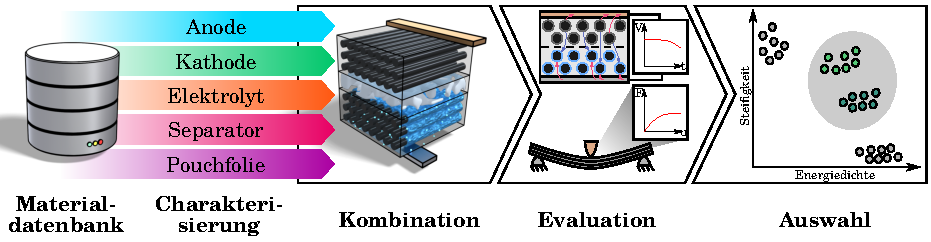
\includegraphics[width=\textwidth, angle=0]{methode.pdf}
		\caption{\label{fig:own_methode}Im Rahmen der Arbeit entwicklete Methode zur Identifizierung von neuen anwendungsspezifischen Strukturbatterien.}
\end{figure}

Die Erarbeitung dieser effizienteren multiphysikalischen Modelle stellen dabei den Ausgangspunkt dieser Arbeit dar. Dabei liegt ein großer Fokus auf der Berücksichtigung auf dem Einfluss von herkömmlichen Elektrolyten und Strukturelektrolyten auf Energiedichte- und Steifigkeitsbetrachtungen. Die Modelle werden anschließen in einem digitalen Framework implementiert. Im Weiteren werden die benötigten Parameter aus der bestehenden Literatur und eigenen Experimenten ermittelt und in einer eigens erstellte Materialdatenbank gesammelt. Aus den verschiedenen Materialien werden durch geeignte Vorauswahlmechanismen die Menge an denkbaren Konfigurationen eingeschränkt. Anschließend wird für jede verbleibende Konfiguration evaluiert und auf ihrer Einsatzszenarien abgeleitet. %Im dritten Schritt werden potenzielle Strukturspeicher mithilfe der validierten Einzelmodelle bewertet und exemplarisch an ausgewählten Kandidaten überprüft. 
Abschleißend werden die bei der Analyse als äußerst vorteilhaften Material- und Parameterkombinationen durch Experimente erprobt und somit eine abschließende Validierung der Methodik erbracht. % dienten \textsc{Kühn} und \textsc{Seidel-Greiff} als Grundlage für ihre experimentellen Untersuchungen, die in der prototypischen Fertigung einer Strukturbatterie kulminierten.

%Mithilfe der entwickelten Methode konnte eine optimierte Strukturbatterie für einen hybriden Anwendungsfall identifiziert werden. Ein erster Funktionsprototyp zeigte eine xx~\% höhere multifunktionale Performanz gegenüber bisher veröffentlichten Strukturbatterien.

% Das zugrundeliegende Prinzip dieses Lösungsansatzes besteht darin, dass Computer besser dazu geeignet sind, eine Vielzahl von einfachen Zusammenhängen zu verarbeiten und dies wiederholt für jede erdenkliche Kombination anzuwenden. Im Gegensatz zu bestehenden Ansätzen beginnt die Modellierung nicht auf atomarer Ebene, sondern auf der Komponentenebene, was eine schnellere Generierung von Ergebnissen ermöglicht. Zudem kann das Modellsystem leicht um Modelle auf mikro- oder molekularer Ebene erweitert werden, um zusätzliche Einflussfaktoren zu berücksichtigen.


%**************************************************************
%                   LITERATURÜBERSICHT  
%**************************************************************
\section{\label{sec:Literaturübersicht}Literaturübersicht}
% 3-5 Seiten

\subsection*{Existierende Strukturbatteriekonzepte}

\begin{figure}[ht]
	%\raggedleft
		%\def\svgwidth{\columnwidth}
        \center
	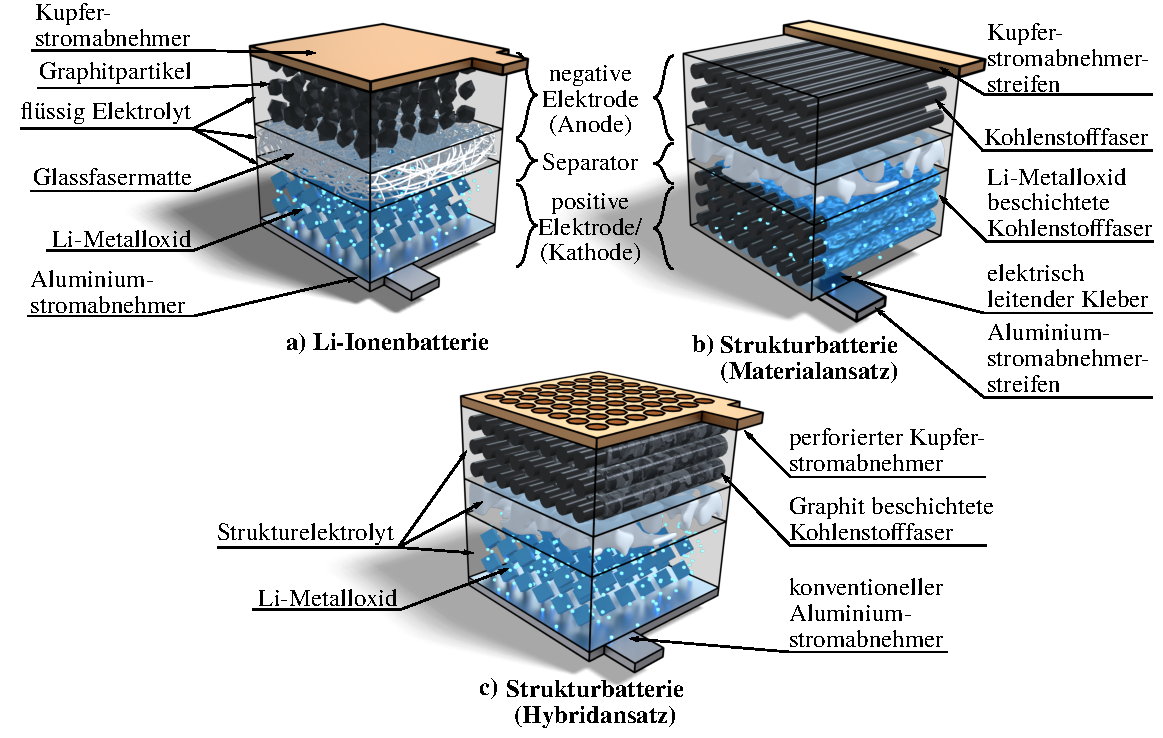
\includegraphics[width=\textwidth, angle=0]{sb_types.pdf}
		\caption{\label{fig:sb_types}Vereinfachte Darstellung von a) konventionellen Li-Ionen Batterie, b) einer Strukturbatterie als multifunktionales Material und c) als multifunktionale Struktur.}
\end{figure}

Die erste multifunktionale Strukturbatterie wurde 2004 von \textsc{Wetzel et al.} im Army Research Laboratories (ARL) der USA entwickelt \cite{Wetzel2004, Snyder2006, Wong2007, Snyder2007}. Die Strukturbatterie Verbundmaterialien basierten auf Kohlenstofffasern als Anode, einer mit $\text{LiFePO}_\text{4}$ beschichteten Edelstahlkathode und einer Glasfasermatte als Separator \cite{Wong2007}. Dieser Aufbau zeigte bereits gute mechanische Eigenschaften. Allerdings konnten die elektrochemischen Eigenschaften wegen auftretender Kurzschlüsse nicht abschließend bestimmt werden.

2009 konzeptionierten \textsc{Liu et al.} \cite{Liu2009} die erste kurzfaserverstärkte Elektrode mit einem festen Polymerelektrolyt als Matrixmaterial. Allerdings konnte die faserverstärkte Elektrode nicht herstellt werden und keinen Feststoffelektrolyten mit ausreichender Ionenleitfähigkeit gefunden werden, weshalb schließlich auf ein gelbasiertes Elektrolyt mit festen und flüssigen Phasenanteilen umgeschwenkt wurde. Da aufgrund der besseren Ionenleitfähigkeit weniger Elektrolyt eingesetzt werden musste, konnte eine Energiedichte von 35~$\si{\watt \hour \per \kg}$ erreicht werden. Durch die fehlende strukturelle Verstärkung wurde allerdings nur ein geringer E-Modul von 3~GPa erreicht.

Der Ansatz der Verwendung von Gelelektrolyten wurde von \textsc{Ekstedt et al.} verfolgt \cite{Ekstedt2010}, in das erstmals ein Kohlenstofffasergewebe als Elektrode einbettet wurde. Ähnlich wie in den Arbeiten von \textsc{Wetzel et al.} wurde auch hier ein glasfaserbasierter Separator und eine mit $\text{LiFePO}_\text{4}$ beschichtete, gewebte Aluminiumfasermatte als Kathode verwendet. Die resultierende Batterie zeichnete sich durch eine Zellspannung von 3,3~V aus. Allerdings wurden die mechanischen und elektrochemischen Eigenschaften nur theoretisch ermittelt.

Im Jahr 2011 präsentierten \textsc{Carlson et al.} \cite{Carlson2011} eine der ersten funktionierenden Strukturbatterien mit einer laminatartigen Struktur. Diese bestand aus einem IMS65-Kohlenstofffasergewebe als Anode, einem Gelelektrolyt, einem Glasfaserseparator und einer mit $\text{LiFePO}_\text{4}$ beschichteten gewebten Aluminiumfolie. Die speicherbare elektrische Energie betrug 0,0247~$\si{\watt \hour \per \kg}$, was ausreichte, um eine LED 70~s lang zu einem schwachen Leuchten zu bringen.

Zwei Jahre später wurden \textsc{Asp et al.} \cite{Asp2013US,Asp2013CN} zwei Patente zugesprochen, die einen Ansatz beschreiben, durch gezielte Funktionalisierung der Faseroberflächen jede Kohlenstofffaser zu einer Elektrode zu machen. Auch wenn die Patente seit 2017 nicht mehr verfolgt werden, wurde darauf aufbauend eine Batterie entwickelt, mit der eine Energiedichte von 10~$\si{\watt \hour \per \kg}$ erzielt wurde. Die theoretisch möglichen 175~$\si{\watt \hour \per \kg}$ bei einem gleichzeitigen Schubmodul von 1~GPa wurden jedoch noch nicht ansatzweise erreicht \cite{Leijonmarck2013, Carlson2013}.

2018 untersuchte \textsc{Meng et al.} \cite{Meng2018} erstmalig den Einsatz von vertikal ausgerichteten Karbonnanoröhrchen (CNT). Diese wurden für die Elektrode auf ein Edelstahlnetz aufgedampft. Anschließend wurde für die Anode $\text{NiO}_\text{x}$ durch einen elektrochemischen Ausscheidungsprozess auf die CNT-Edelstahlelektrode eingelagert. Mit dem gleichen Verfahren wurde $\text{FeO}_\text{x}$ für die Kathode aufgetragen. Die Strukturbatterie erreichte dabei eine Zugsteifigkeit von 7,0~GPa und eine Energiedichte von 1.4~$\si{\watt \hour \per \kg}$.

\textsc{Moyer et al.} \cite{Moyer2020} modifizierten den für Batterien typischen Pouchzellenansatz, indem das verpresste Kohlenstofffasergewebe gleichzeitig als Stromkollektor und Schutzfolie dient. Durch das anodenseitige Aufbringen von Graphit und $\text{LiFePO}_\text{4}$ auf der Kathode nehmen die Fasern jedoch nicht direkt am chemischen Prozess teil. Durch das bessere, als Interkalation bezeichnete, Ionen-Einlagerungsverhalten bei Graphit konnte eine hohe Energiedichte von 35~$\si{\watt \hour \per \kg}$ gemessen werden. Jedoch führte der Ansatz zu einer vergleichsweise geringen Zugsteifigkeit von 2~GPa.

\textsc{Thakur \& Dong} \cite{Thakur2020} stellten 2020 die erste 3D-gedruckte Strukturbatterie her. Mithilfe eines Koextrusionsprozesses konnte eine Kohlenstofffaser, die vorher mit einem festen Polymerelektrolyten beschichtet wurde, zusammen mit einem Li-gedopten Polylactide-Matrixmaterial aufgebracht werden. Nach dem Drucken der Elektrode wurde manuell eine Glasfasermatte und abschließend eine Aluminiumfolie als Kathode aufgebracht. Neben der Möglichkeit, neue Batteriegeometrien zu drucken, wurde auch durch die höhere Dichte an Aktivmaterial in Fasernähe eine vergleichsweise hohe Energiedichte von 24~$\si{\watt \hour \per \kg}$ erreicht. Allerdings konnte durch den geringen Faservolumenanteil ein niedriges Zugmodul von 0.29~GPa gemessen werden.

2021 präsentierte \textsc{Asp et al.} \cite{Asp2021} ein Design mit unidirektionalen Kohlenstofffasern als Anode, einem gewebten Glasfaserseparator und einer $\text{LiFePO}_\text{4}$-beschichteten Aluminiumplatte als Kathode. Durch ein verbessertes Herstellungsverfahren und eine günstige Faseranordnung konnte ein E-Modul von 25~GPa und eine Zugfestigkeit von 300~MPa gemessen werden. Gleichzeitig erreichte die Strukturbatterie eine Energiedichte von 24~$\si{\watt \hour \per \kg}$. \textsc{Siraj et al.} \cite{Siraj2023} verbesserten zwei Jahre später den Infiltrationsprozess, wodurch sie bei annähernd gleichbleibenden mechanischen Eigenschaften die Energiedichte auf nahezu 41~$\si{\watt \hour \per \kg}$ verdoppeln konnten.

\begin{table}[ht]
    \centering
    \caption{Auswahl realisierter Strukturbatterien}
    \begin{tabular}[t]{m{0.15\textwidth} m{0.15\textwidth}<{\centering} m{0.15\textwidth}<{\centering} m{0.2\textwidth}<{\centering} m{0.1\textwidth}<{\centering} m{0.1\textwidth}<{\centering}}
    \toprule
    &Elastizitäts-modul~[GPa]&Energie-dichte~[Wh/kg]&Struktur-batterieart&Jahr&Referenz\\
    \midrule
    \textsc{Wong et al.}&8&/&Edelstahlbatterie&2007&\cite{Wong2007}\\
    \textsc{Liu et al.}&3&35&Faserbatterie&2009&\cite{Liu2009}\\
    \textsc{Meng et al.}&7&4&Edelstahlelektroden&2018&\cite{Meng2018}\\
    \textsc{Moyer et al.}&35&2&Kohlenstofffaser-verbund&2020&\cite{Moyer2020}\\
    \textsc{Thakur et Dong}&0.29&24&Faserbatterie&2020&\cite{Thakur2020}\\
    \textsc{Huang et al.}&9.2&43&Edelstahlelektroden&2020&\cite{Huang2020}\\
    \textsc{Asp et al.}&25&24&Kohlenstofffaser-verbund&2021&\cite{Asp2021} \\
    \textsc{Saraj et al.}&26&41&Kohlenstofffaser-verbund&2023&\cite{Siraj2023}\\
    \bottomrule
    \end{tabular}
\end{table}%

Die existierenden Studien an Strukturbatterien zeigen einen starken Fokus auf geschichtete Bauweisen, die sich an die Struktur von herkömmlichen Lithiumionenbatterien anlehnt, siehe Bild~\ref{fig:sb_types}a,b. Aus den bisherigen Ergebnissen leiten sich außerdem eine Reihe an Verbesserungspotenzialen für weitere Forschungen ab. Die größte Herausforderung stellt bislang das Erzielen einer möglichst guten Lithium-Interkalation in das Aktivmaterial der Elektrode dar. Das Gleiche gilt für die Lithiummigration zwischen den beiden Elektroden über den Strukturelektrolyt, welche möglichst unbehindert, bei gleichzeitiger Beibehaltung der mechanischen Steifigkeit und Festigkeit,  stattfinden muss~\cite{Asp2015}. Besonders zur weiteren Eröhung der Energiedichte, sind neue Ansätzte wie perforierte Stromabenehmer, Seperatorfreie Bauweisen durch Strukturelektorlyt oder hybride Bauweisen für bessere zellchemie denkbar, siehe Bild~\ref{fig:sb_types}c. Die Wichtigkeit solcher Verbesserungen wird dadurch verstärkt, dass die aktuell höchste erreichte Energiedichte von 41~$\si{\watt \hour \per \kg}$ am unteren Ende der benötigten Energiedichte, die für den Einsatz in z.B. Elektrofahrzeugen erforderlich ist, liegt. Diese Mindestgrenze der Energiedichte wurde allerdings 2022 von dem Forschungsteam um \textsc{Linde} am Deutschen Zentrum für Luft- und Raumfahrt (DLR) weiter angehoben auf 74~$\si{\watt \hour \per \kg}$, bei einem gleichzeitig Mindest-E-Modul von 54~GPa und einer Mindestfestigkeit von 203~MPa, sowie einer Leistungsdichte von 376~W/kg ~\cite{Ishfaq2022}. Womit ein Durchbruch für Strukturbatterien im Sinne einer industriellen Anwendung noch aus steht.

\subsection*{Modellierung des gekoppelten elektrochemischen und mechanischen Verhaltens von Strukturbatterien}

Über jedes Material was in einer heutigen sicherheitsrelevanten Anwendung verwendet wird muss ausreichendes Wissen existieren um das Verhalten im Belastungsfall ausreichend vorherzusagen. Bei Strukturbatterien besteht die Herausforderung nicht sowohl die elektrochemsichen und mechansichen Prozesse einzeln zu verstehen, sondern auch dabei ihre gegenseitigen Wechselwirkungen zu berücksichtigen~\cite{Carlstedt2022a}. Diese Schwierigkeiten werden durch den hohen Multifunktionalitätsgrad von Material und Struktur zu einem .

Eine vergleichsweise einfache Beschreibung der elektrochemischen und thermischen Phänomenen kann durch äquivalente Ersatzschaltungen (\textit{engl.} equivalent circuit model, ECM) erfolgen \cite{Bavsic2022}. Bereits mit wenigen Elementen lassen sich Spannungsänderungen in Abhängigkeit vom Lade- und Entladeverhalten gut annähern \cite{YannLiaw2004}. Durch zusätzliche Erweiterungen lassen sich auch Alterung und der Einfluss zahlreicher thermischer Effekte berücksichtigen \cite{Hannan2017,Tran2021}. Aufgrund des geringen Rechenaufwands eignen sich diese Modelle besonders gut für zeitkritische Anwendungen wie die Lade- und Entladeregelung, siehe Abbildung~\ref{fig:battery_modelling_in_context}. Die Modellparameter müssen jedoch jedes Mal durch einen Fittingprozess für das jeweilige System bestimmt werden \cite{Tomasov2019}. Eine Verknüpfung der einzelnen Schaltelemente mit realphysikalischen Größen war bisher nur wenig erfolgreich \cite{Plett2015}.
\begin{figure}[ht]
	%\raggedleft
		%\def\svgwidth{\columnwidth}
        \center
	\includegraphics[width=\textwidth, angle=0]{batterie_modelling_approaches.pdf}
		\caption{\label{fig:battery_modelling_in_context}Übersicht der Batteriemodellierung im Kontext neuer Batterieentwicklungen.}
\end{figure}
Die physikalische Modellierung der elektrochemischen Phänomene wurde maßgeblich von \textsc{Doyle} \cite{Doyle1995,Doyle2003,Ceder2002}, \textsc{Fuller} \cite{Fuller2018,Takeuchi2008} und \textsc{Newman} \cite{Doyle1995,Newman2021} vorangetrieben. Das von ihnen entwickelte und nach ihnen benannte DFN-Modell (alternativ auch \textit{pseudo zwei dimensionale} (P2D) Modell genannt) \cite{Doyle1993} beschreibt die Prozesse auf der Makroskala und eignet sich daher sehr gut, um die Vorgänge auf Zellebene zu modellieren. Die benötigten Parameter können durch Experimente oder mithilfe von Simulationen auf niedrigeren Skalen wie der Dichtefunktionaltheorie (DFT) oder molekulardynamischen (MD) Simulationen bestimmt werden \cite{Chen2022}. Das DFN-Modell findet heute weitreichenden Einsatz und wurde seit seiner Veröffentlichung im Jahr 1993 zahlreich modifiziert und erweitert. Einige der bekanntesten Derivate sind das \textit{Single Particle Model} (SPM) \cite{Li2017} und das \textit{full homogenized macro-scale} (FHM) Modell \cite{Arunachalam2019}, welche beide darauf abzielen, die sehr rechenintensiven Differentialgleichungen in ihrer Komplexität zu reduzieren.

Die Kopplung mit thermischen Prozessen wurde bereits 1995 von \textsc{Pals et Newman} \cite{Pals1995,Pals1995a} begonnen und seitdem kontinuierlich weiterentwickelt \cite{Chen2005,Onda2006,Kim2013,Gao2021,Liu2023}. Auch der Einfluss der lithierungsbedingten Ausdehnung \cite{Bower2011,Yang2014,Roberts2014,Pereira2019,Mai2019,Li2020,Hoeschele2023}, Rissbildung \cite{Dionisi2017,Wang2020a,Pistorio2023} und Alterung \cite{RedondoIglesias2020} wurden in zahlreichen Studien untersucht. Zusätzlich existieren viele Studien, die sich einer vereinheitlichten Modellierung aller Effekte \cite{Wu2014,Kim2018,Liu2020,Yin2020} und auch einer Modellierung über mehrere Größenskalen hinweg widmen \cite{Liu2019,Li2020a,Katrasnik2021}.

\textsc{Carlstedt} erarbeitete stückweise in einer Reihe von Beiträgen eine Koppelung von Elektrochemie, Mechanik und Thermodynamik, um das Verhalten von Strukturbatterien zu beschreiben \cite{Carlstedt2019,Carlstedt2019a,Carlstedt2019b,Carlstedt2020,Carlstedt2020b,Carlstedt2022,Carlstedt2022a,Carlstedt2022b}. Auch wurde der Ansatz um den nicht-linearen Zusammenhang durch die Gestaltänderung von \textsc{Larsson et al.} \cite{Larsson2023} erweitert.

\subsection*{Modelierungsgetriebene Entwicklung von neuen Batterien und Strukturbatterien}

Die neu motivierte Forschung in bereits untersuchte und neue Batteriematerialien baut aktuell hauptsächlich auf theoretischen Überlegungen und experimentellen Prototypen auf. Um die Vielzahl an Effekten zu berücksichtigen und der enormen Anzahl an vielversprechenden Materialkombinationen Herr zu werden, argumentierten \textsc{Greenhalgh} \cite{Greenhalgh2024,Greenhalgh2024a} und \textsc{Asp} \cite{Asp2024} auf dem \textsc{1st Structural Power Research Showcase} in London, dass nur durch intensive Modellierungsarbeit diese Varianten voruntersucht und ausreichend eingeschränkt werden können. Der multiphysikalische Modellierungsansatz von \textsc{Carlstedt} wird zwar in diesem Zusammenhang oft erwähnt, allerdings sorgen Skalierungseffekte, wie etwa Defekte und Faser-Matrix-Interfaceeffekte, die besonders bei Oberflächenmodifikation von Kohlenstofffasern sowohl für deutlich andere elektrochemische als auch mechanische Eigenschaften des Verbundes sorgen, für große Ungenauigkeiten bei der Adaption \cite{Franco2019,Fam2024}. Hinzu kommt, dass die Modelle von Carlstedt mit zunehmender Komplexität immer mehr Materialparameter benötigen und bereits jetzt mehr als 20 teils aufwendig zu bestimmende Parameter pro Material erfordern \cite{Greenhalgh2024a}. Bis heute wurde dieser Ansatz daher vor allem zur nachträglichen Validierung und zur detaillierten Untersuchung von sensorischen und aktuatorischen Effekten von Strukturbatterien genutzt \cite{Carlstedt2023}.

Die einzige zurzeit existierende Veröffentlichung zur Vorhersage von Energiedichte und Zugsteifigkeit stammt ebenfalls von \textsc{Carlstedt} \cite{Carlstedt2018}. Jedoch wurde dazu ein in der Komplexität deutlich reduzierter Ansatz verwendet. Hinzu kommt, dass bei der Auswertung nur drei Varianten untersucht wurden, die sich in ihrer Elektrodendicke und dem Volumenanteil des Aktivmaterials unterschieden. Außerdem wurde der Einfluss des Elektrolyten nicht berücksichtigt.



% Dan Zenkert KTH Prof (Fasercehmie), 
% Dr Faye Smith OBE (Director at Avalon Consultancy Services)
% Peter Linde (DLR, CORCER Mitgleid)
% Milo Shaffer ( Professor of Materials Chemistry London)
% Natasha Shirshova (Lecturer in Engineering Materials at Durham University)
% Derrick Fam (Scientist at Institute of Materials Research and Engineering (IMRE), Adjunct Assistant Professor (NTU, MSE), Dy. Dir. Singapore Battery Consortium)
% Alexander Bismarck (Professor of Material Chemistry Wien)
% Madhavi Srinivasan (Professor at Nanyang Technological University Singapore)



   

